% ---------------------------------------------------------------------------
% simulant, ACS Sensors 판본 (2026-11-01 신설)
%
% 왜 새 디렉터리인가. paper/ 는 elsarticle·JHM 판본이고 11,141단어다.
% ACS Sensors 는 Article 권장 8쇄면, 1,000단어/쇄면, 단단 그림 250·양단 500
% 환산이다. 참고문헌 50건이 약 1,300, 도판 4장이 1,500 을 먹으므로 본문
% 예산은 약 5,000단어다. 다듬기가 아니라 재집필이라 판본을 분리한다.
% paper/ 는 그대로 두어 수치 정본과 verify_consistency 의 대조 대상을 유지한다.
%
% 골격은 Ku 제공 ACS 템플릿(phthalate 판본)의 관례를 따른다.
%
% journal 코드 주의. ACS Sensors 의 CODEN 은 ascefj 인데 achemso.cls 의
% 저널 목록에 없다. ascefj 를 넣으면 클래스가 알 수 없는 저널로 처리해
% '(Sub)section ... ignored' 경고를 내며 절 제목을 전부 삼킨다 (2026-11-01
% 적발). 그래서 템플릿과 동일하게 jacsat 을 쓴다. 조판 편의용일 뿐이고
% 투고 대상은 ACS Sensors 다.
%
% 분량 예산 (총 8쇄면 = 8,000 환산)
%   Introduction            700
%   Results and Discussion  2,800
%   Conclusions             400
%   Experimental Section    1,100
%   -------------------------------
%   본문 소계               5,000
%   도판 4장                1,500   (양단 2장 1,000 + 단단 2장 500)
%   참고문헌 50건           1,300
%   -------------------------------
%   합계                    7,800
%
% 컴파일: pdflatex -> bibtex -> pdflatex x2
% ---------------------------------------------------------------------------
\documentclass[journal=jacsat,manuscript=article,margin=1in]{achemso}

\usepackage[T1]{fontenc}
\usepackage{amsmath}
\usepackage{amssymb}
\usepackage{float, graphicx, caption, xcolor}
\usepackage{subcaption}
\captionsetup[sub]{labelformat=parens, labelsep=none, font=bf, position=top}
\usepackage{booktabs}
\usepackage{textcomp}
\usepackage{url}
\usepackage[per-mode=symbol]{siunitx}

%%%%%%%%%%%%%%%%%%%%%%%%%%%%%%%%%%%%%%%%%%%%%%%%%%%%%%%%%%%%%%%%%%%%%
%% Meta-data block
%%%%%%%%%%%%%%%%%%%%%%%%%%%%%%%%%%%%%%%%%%%%%%%%%%%%%%%%%%%%%%%%%%%%%
% 2026-11-01 Ku 확정. 종전(2026-10-24)과 다른 점은 공동1저자 해제(Ku 단독)와
% Doo-Hee Lee 의 교신 해제 둘뿐이고, 인원과 소속은 10-24 판 그대로다.
% Jeongyun Kim 은 이 원고 한정으로 CBRN 소속 표기 (Ku 지시).
\author{Ku Kang}
\affiliation[CBDRI]{Chemical, Biological, Radiological and Nuclear (CBRN)
Defense Research Institute, Ministry of National Defense, Seoul, Republic of
Korea}

\author{Jeongyun Kim}
\affiliation[CBDRI]{Chemical, Biological, Radiological and Nuclear (CBRN)
Defense Research Institute, Ministry of National Defense, Seoul, Republic of
Korea}

\author{Miae Kim}
\affiliation[CBDRI]{Chemical, Biological, Radiological and Nuclear (CBRN)
Defense Research Institute, Ministry of National Defense, Seoul, Republic of
Korea}

\author{Doo-Hee Lee}
\affiliation[KMA]{Department of Civil Engineering and Environmental Sciences,
Korea Military Academy, Seoul 01805, Republic of Korea}

\author{Jin Yoo}
\affiliation[CBDRI]{Chemical, Biological, Radiological and Nuclear (CBRN)
Defense Research Institute, Ministry of National Defense, Seoul, Republic of
Korea}

\author{Yoon Jeong Jang}
\affiliation[CBDRI]{Chemical, Biological, Radiological and Nuclear (CBRN)
Defense Research Institute, Ministry of National Defense, Seoul, Republic of
Korea}
\email{yjjangchem@korea.kr}

% ORCID (ACS Paragon Plus 제출 시 입력. 본문에는 넣지 않는다):
%   Ku Kang          0000-0001-8739-218X   bisu9082@mnd.go.kr
%   Jeongyun Kim     0009-0004-1377-8572   kimjy3022@snu.ac.kr
%   Miae Kim         없음                  kma9292@daum.net
%   Doo-Hee Lee      0000-0002-5116-2064   dooheelee@korea.kr
%   Jin Yoo          0000-0002-7738-8424   tysonyj@snu.ac.kr
%   Yoon Jeong Jang  0000-0002-5625-2528   yjjangchem@korea.kr

\title{Descriptor Similarity Does Not Predict Array Response: Chemical
Warfare Agent Simulants Tested Against Seventeen Authentic Agents}

\keywords{chemical warfare agents, simulants, colorimetric sensor array,
surrogate validation, permutation test, applicability domain}

\begin{document}

%%%%%%%%%%%%%%%%%%%%%%%%%%%%%%%%%%%%%%%%%%%%%%%%%%%%%%%%%%%%%%%%%%%%%
%% TOC graphic. 길이 환산에서 제외된다.
%% TODO 현재 것은 JHM 프레임(서술자공간 중심)으로 그린 구판이다.
%% 응답공간 헤드라인에 맞춰 다시 그려야 한다.
%%%%%%%%%%%%%%%%%%%%%%%%%%%%%%%%%%%%%%%%%%%%%%%%%%%%%%%%%%%%%%%%%%%%%
\begin{tocentry}
  \centering
  % ACS TOC 규격은 최대 8.25 x 4.45 cm. 현재 도판 비율 2.40 이므로
  % 8.25cm 폭에서 높이 3.44cm, 규격 안에 든다.
  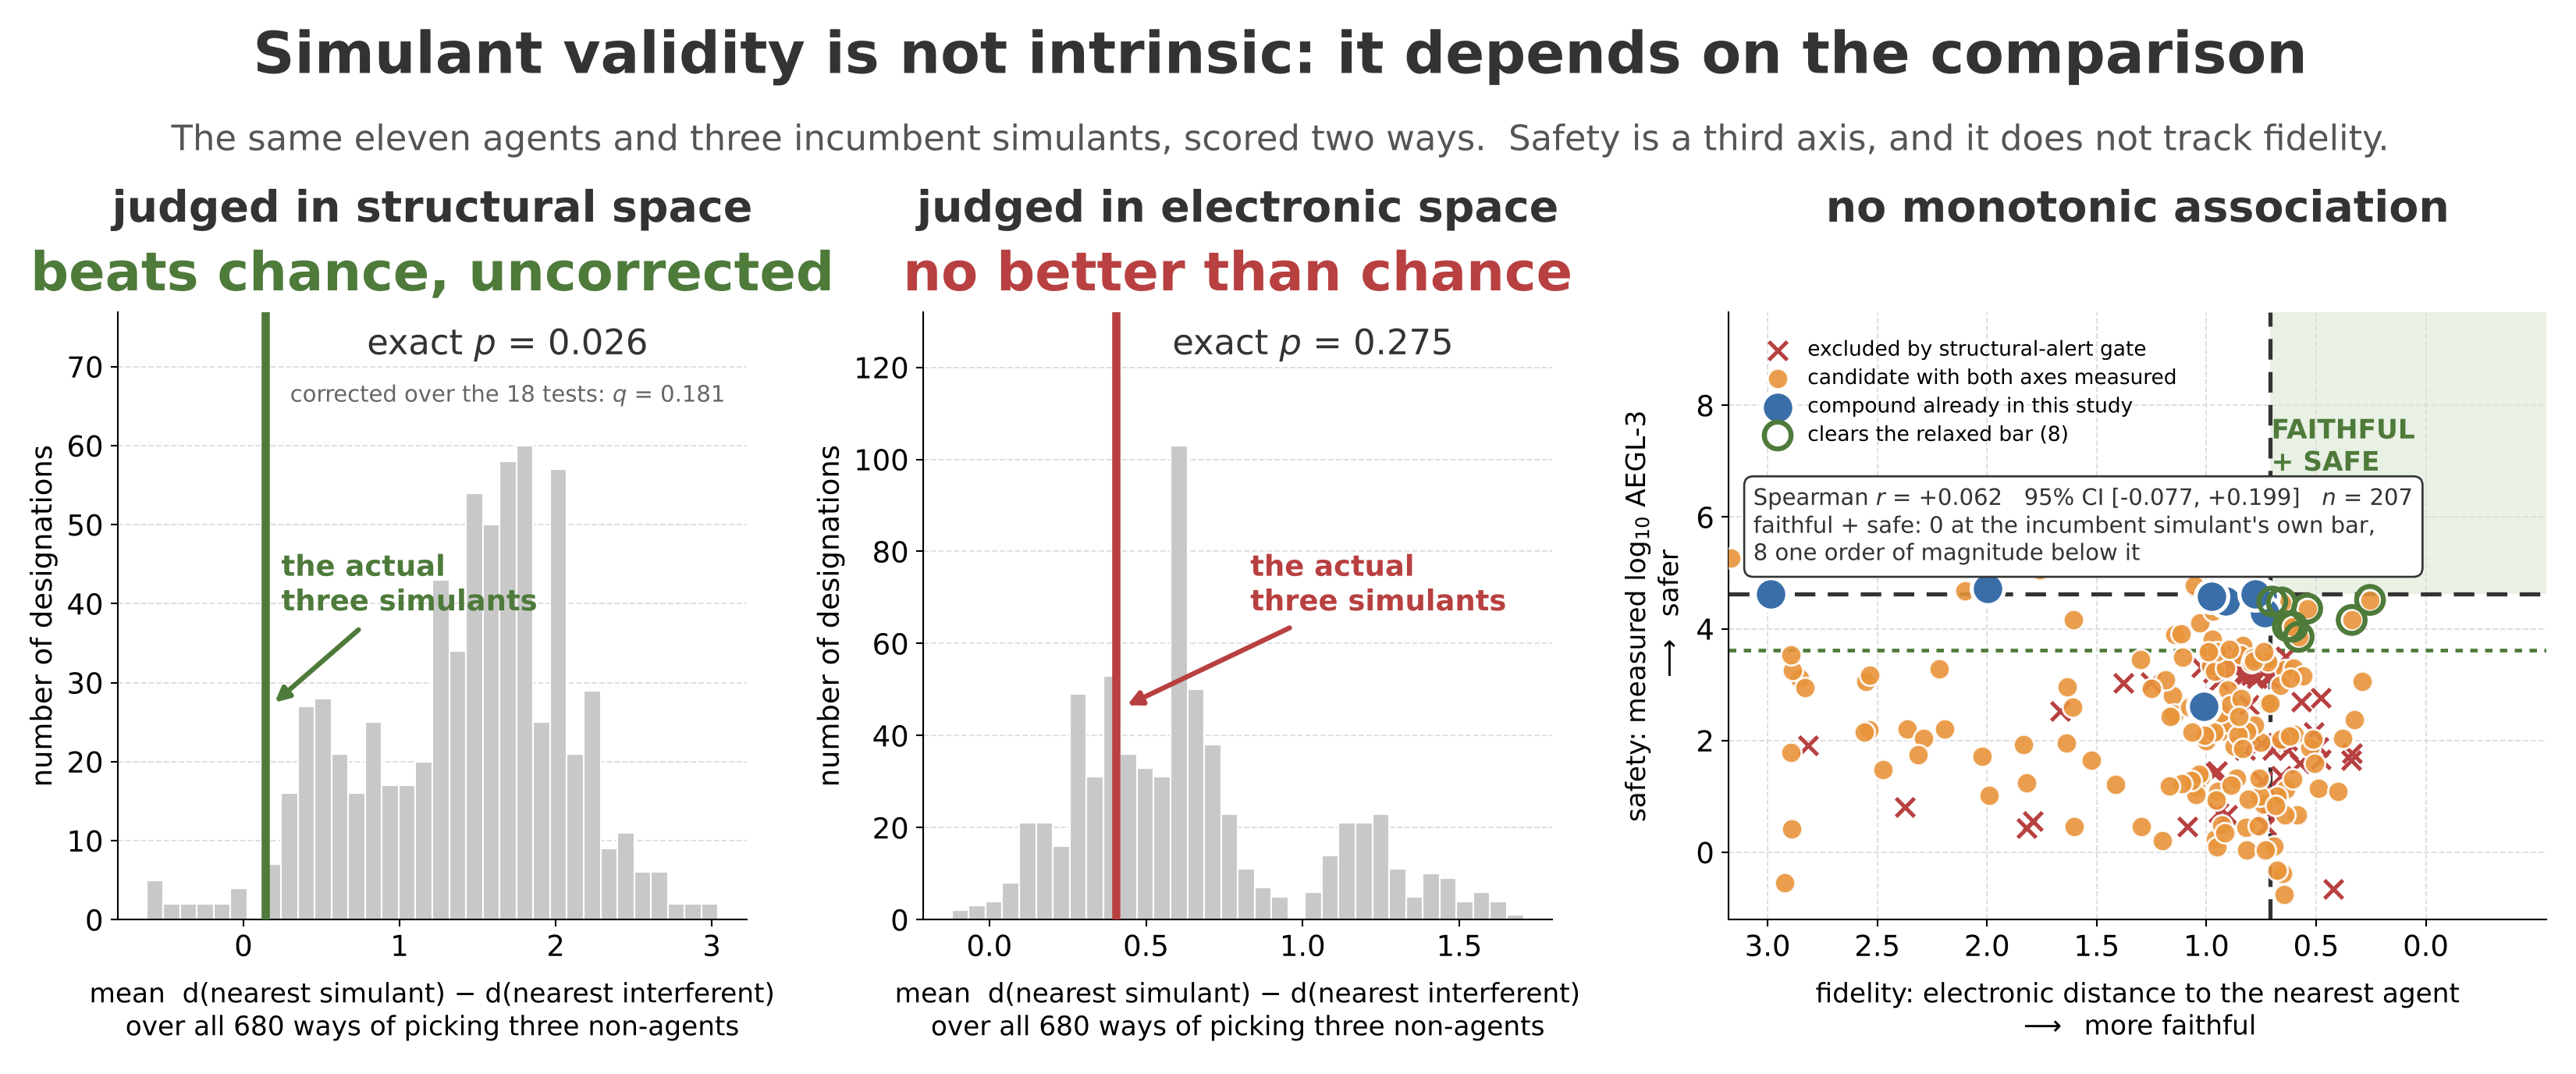
\includegraphics[width=8.25cm]{graphical_abstract.png}
\end{tocentry}

% --- Abstract: ACS Sensors 는 80~250 단어. 목적 1문장, 방법 2~3문장,
%     결과 2~3문장 구조를 요구한다. 현재 228단어.
\begin{abstract}
Chemical warfare agent detection is developed and qualified on simulants,
and we asked what measurement establishes that a simulant reproduces the
agent it stands in for. A 29-dye colorimetric array was used to measure
seventeen authentic agents, spanning nerve, blood, choking, vesicant and
A-series compounds, at five concentrations in two optical channels, and the
resulting response patterns were compared with the molecular-descriptor
distances on which simulant selection in practice rests. Agreement was
tested by exact Mantel permutation within each run, by exact enumeration of
all 680 possible simulant designations in descriptor space, and against
permutation nulls built for each comparison. The array separates compounds
in all six run-channel cells, with $p$ from $4.6\times10^{-8}$ to 0.025, so
the measurement is sound. Descriptor distance nonetheless fails to predict
response distance: twelve exact Mantel tests and six combinations of them
leave nothing below $q=0.05$. Dimethyl methylphosphonate, the standard
G-agent simulant and the benchmark compound for decontamination efficiency,
is anti-correlated with soman and cyclosarin in the ultraviolet channel, and
its correlation with sarin falls from $+0.77$ at 500~ppm to $+0.36$ at
10~ppm, the end at which point detectors operate. Across the seventeen
agents measured, exactly one designated simulant has ever been measured
beside them.
\end{abstract}

\section{Introduction}
% 예산 700단어. 현재 411단어.
% 이 절이 하는 일 둘. (1) 센서 개발자의 언어로 공백을 세운다.
% (2) 거부 조항 "deals with known sensing concepts and does not offer a
% significant, original application of the method" 를 선제 차단한다.

Nearly every chemical warfare agent detector in the literature is developed,
optimised and qualified on compounds that are not chemical warfare
agents.\cite{askim2013,rakow2000} Dimethyl methylphosphonate stands in for
the G-series nerve agents,\cite{niosh2002simulant} dipropylene glycol
monomethyl ether for training detectors,\cite{seitzinger2006simulant} and
methyl salicylate for vapour penetration through protective
ensembles.\cite{nrc1997mist,astmf2588} The substitution is unavoidable,
because the agents are lethal at concentrations where handling them requires
a licensed facility, and it is load-bearing: a sensor reported as selective
for sarin has, in most cases, never been exposed to sarin.

What licenses the substitution is a claim of similarity. The compound chosen
is said to be agent-like, and similarity is read from molecular
descriptors: vapour pressure, dipole moment, frontier orbital energies,
substructure and shape. The claim that matters for a detector is different.
It is that the substitute produces the response the agent would produce in
the same device. Those two claims are connected only if descriptor
similarity transfers to response similarity, and that transfer has not been
measured.

It has not been measured because measuring it requires the agents. Response
data on authentic agents exist in few places, and the compounds used as
simulants are rarely run alongside them. A recent survey of the field found
no standard for chemical warfare agent simulants at all, and recorded that
they have generally been selected on the basis of their historical
use.\cite{lawrence2025simulants} Our institute is an OPCW designated
laboratory, which identifies and assays authentic agents under an accredited
procedure, so the comparison can be made on the agents themselves.

This work reports that measurement. A 29-dye colorimetric array was used to
record the responses of seventeen authentic agents at five concentrations in
two optical channels, and those responses were compared against the
molecular-descriptor distances that simulant selection relies on. The array
separates compounds in every run and channel, so the measurement is sound.
Descriptor distance nonetheless carries no detectable information about
response distance. Dimethyl methylphosphonate, the compound the field treats
as the G-agent surrogate, is anti-correlated with two of the four G agents,
and its resemblance to sarin weakens as the concentration falls towards the
range where point detectors operate. Where the designation record and a
regulatory toxicity model might have supplied the missing evidence, both are
empty for the same compounds.

% 기여 선언. 거부 조항을 겨냥한 단락이므로 지우지 말 것.
This is not a new sensing method, and we propose no replacement compound.
It is a measurement of whether the substitutes the field already relies on
carry the property they are relied upon for.

% ===========================================================================
\section{Results and Discussion}
% 예산 2,800단어.

\subsection{The array separates the agents}
% 예산 400단어. 현재 약 400단어.

A comparison between descriptor space and response space is worth making
only if the response measurement resolves the compounds at all. We checked
that first. Each exposure gives a 29-dye $\Delta E$ vector, which we centred
dye-wise at each concentration and normalised to unit length, so that the
comparison is between response patterns rather than response magnitudes.
Agreement was then measured as the cosine between patterns, within
replicates of one compound and between different compounds.

\begin{figure}[htb]
  \centering
  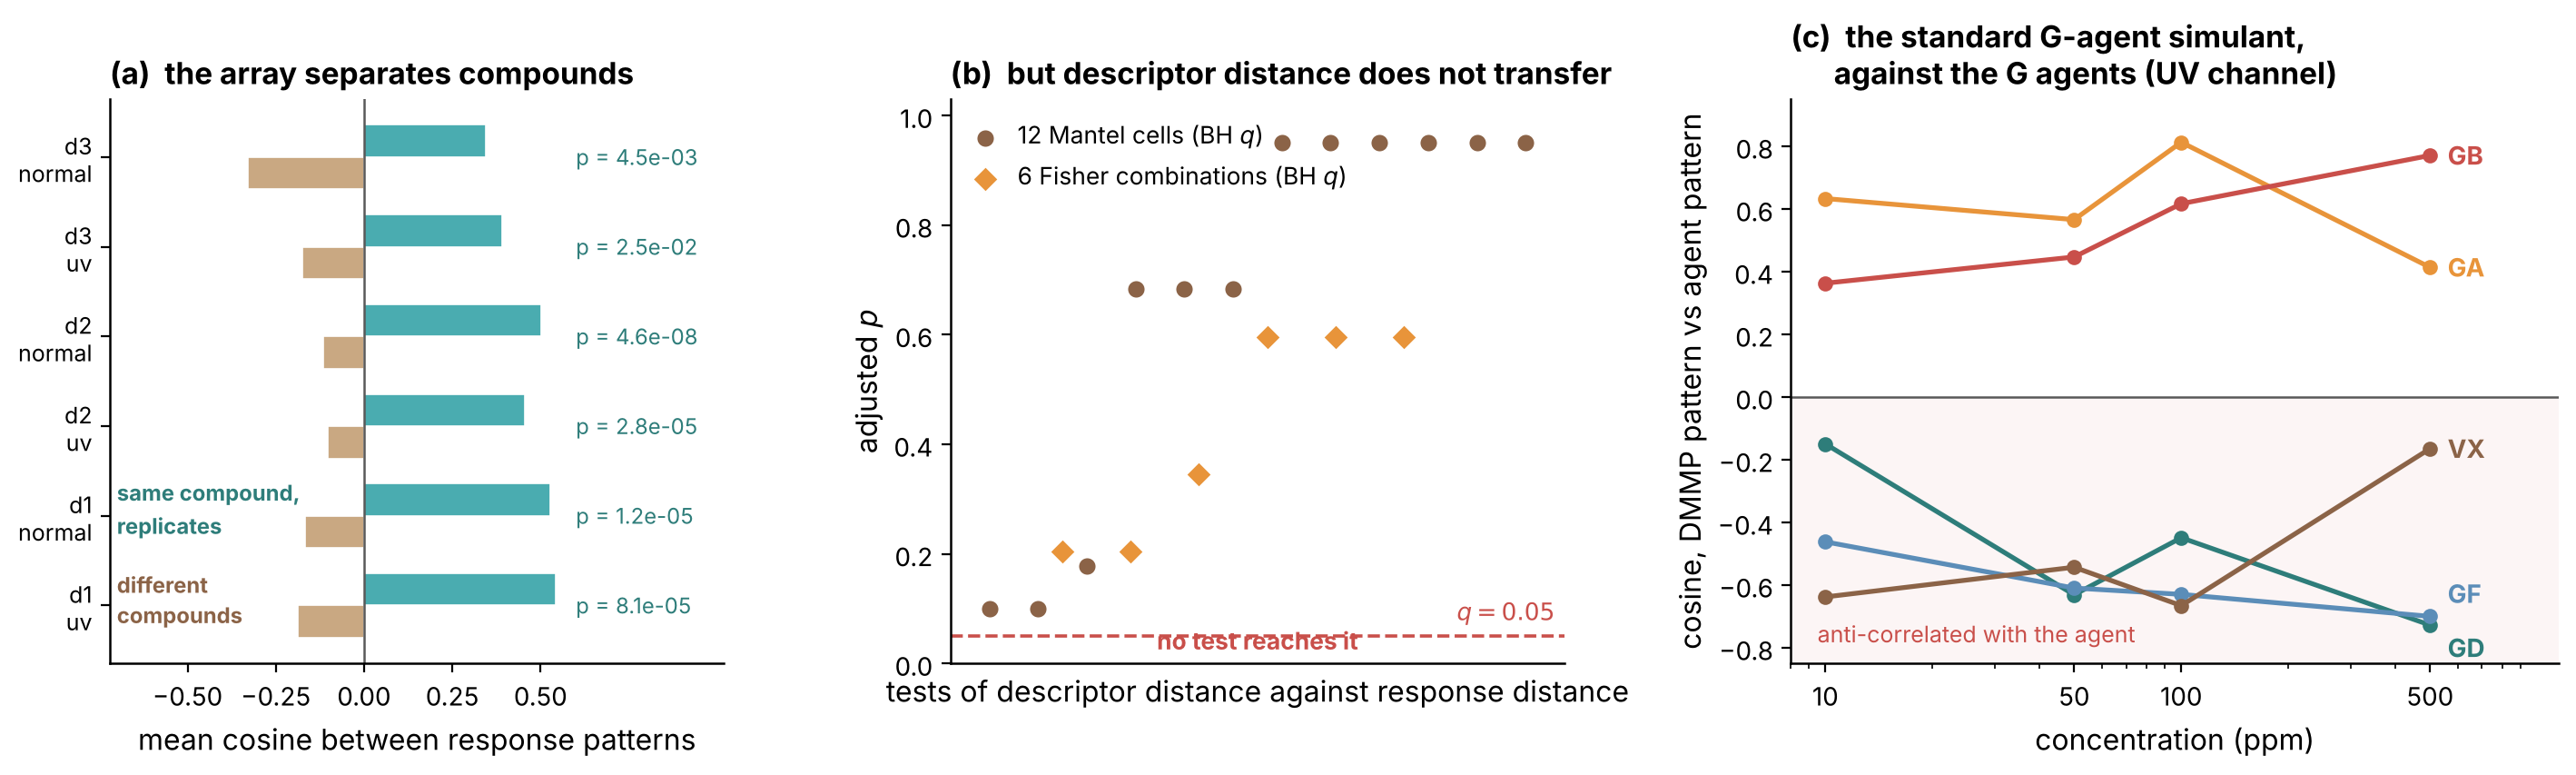
\includegraphics[width=\textwidth]{Fig_talk_response.png}
  \caption{Response-space tests on authentic agents. (a) Mean cosine
  between response patterns, within replicates of the same compound and
  between different compounds, for three runs in two optical channels.
  (b) Adjusted $p$ for every test of descriptor distance against response
  distance: twelve exact Mantel cells and six Fisher combinations of the
  independent runs. (c) Cosine between the response pattern of DMMP and
  those of the four G agents and VX, by concentration, in the ultraviolet
  channel.}
  \label{fig:response}
\end{figure}

The array resolves the compounds in every run and channel
(Figure~\ref{fig:response}a). Replicates of one compound correlate at
$+0.345$ to $+0.542$, different compounds anti-correlate at $-0.103$ to
$-0.330$, and the separation holds in all six run-channel cells, with $p$
from $4.6\times10^{-8}$ to 0.025.

Two limits on that statement belong here rather than in the Supporting
Information. The first is that dye-wise centring forces the mean
between-compound cosine towards an algebraic floor of $-1/(n-1)$, and the
observed means clear that floor by only 0.013 to 0.064 across the four
cells where it could be evaluated. Most of the apparent separation is
therefore a property of the centring, and what the test establishes is the
weaker statement that replicate agreement exceeds between-compound
agreement. The second is that six dye columns in the ultraviolet pivot of
the second run were bit-identical across every row. Tracing them to the
source images showed that those dyes do not fluoresce under ultraviolet
excitation and the regions of interest had read plate background, so one
channel had been recorded six times. Columns identical across all rows are
counted once, which leaves 23 effective channels in that cell and 25 in the
ultraviolet pivot of the third run.

\subsection{Descriptor distance does not predict response distance}
% 예산 700단어. 현재 약 650단어.

Simulant selection rests on an implicit transfer: that a compound close to
an agent in descriptor space will be close to it in whatever the detector
measures. We tested the transfer directly, as the agreement between two
distance matrices over the same compounds, one built from descriptors and
one from response patterns. Agreement was measured by Mantel correlation
and referred to a null built by enumerating every relabelling of the
compounds, so the test is exact rather than sampled.

The test is run within each run and never across runs. The three runs share
no compound, so the dye-wise sensitivity of one plate cannot be calibrated
against another, and pooling responses across them would require a
commutability assumption we cannot support. That restriction sets the
power. Six compounds in the first run and six in the second carry both a
response pattern and a descriptor vector, giving fifteen pairs in each,
and the third run drops out because the A-series compounds are not in the
descriptor panel. Nitrogen mustard drops out of the second run for the same
reason.

Across the twelve cells, three spaces by two channels by two runs, nothing
survives correction (Figure~\ref{fig:response}b). Three cells reach a
nominal $p$ below 0.05, all of them in the second run: the merged space in
the ultraviolet channel at 0.0153, the structural space in the same channel
at 0.0167, and the electronic space in the reflectance channel at 0.0444.
Benjamini--Hochberg correction over the twelve leaves a smallest adjusted
value of 0.10. The pattern of the three is itself uninformative about
transfer, because the two ultraviolet cells implicate the structural and
merged spaces while the reflectance cell implicates the electronic space,
and the same space does not reproduce across channels of the same plate.

Combining runs does not change the answer. The first and second runs share
neither compounds nor plates, so their exact Mantel $p$ values are
independent and can be combined by Fisher's method. We report all six
combinations of three spaces and two channels rather than selecting one,
which would reintroduce the analyst freedom the test is meant to remove.
The smallest adjusted value over the six is 0.204, and none reaches 0.05.

What this does not license is the claim that no transfer exists. Fifteen
pairs is a weak test, and the pooled rank correlations are correspondingly
imprecise: the structural space in the ultraviolet channel gives
$\rho=+0.31$ with a 95\% interval from $-0.45$ to $+0.81$, which excludes
neither zero nor a strong association. The defensible statement is that the
transfer on which simulant selection depends has not been established, in
the one body of authentic-agent response data where it could be tested, and
that the experiment which would settle it is a run containing a compound
already measured in an existing run. Such a bridge would fix the plate
correction and open the 136 cross-run pairs that are closed today.

\subsection{The standard G-agent simulant against the G agents}
% 예산 700단어. DMMP 코사인 GA +0.76 GB +0.65 GD -0.49 GF -0.72 VX -0.70.
% 농도 의존(GB 0.363 -> 0.771), 4! 전수 p 하한 0.083, BH 10건 q_min 0.28.
% 귀무 대조 둘을 여기서 전부 보고한다: 순위 1위 2/10 대 기대 2.0
% (이항 p 0.624), 염료 집중도가 작용제-작용제 쌍·치환 귀무와 같음.
% 도판: Fig 2.

\subsection{Descriptor space cannot supply the missing validation}
% 예산 600단어. 35종 0/11 전 검정 비유의, 28종 4/11 명목 0.0250,
% BH-18 0.181, 부분공간 백분위 24.3, 지정 순위 5/680 p 0.0074.
% 도판: Fig 3.

\subsection{Neither the designation record nor a toxicity model fills the gap}
% 예산 400단어. NIOSH 여과재 파과(자체 면책 문구 포함), DPGME 훈련용 IMS,
% DCM 전거 없음. AEGL 1/3, QSAR 20/20 일방 실패, 적용영역 안 최악 482배.
% 도판: Fig 4.

% ===========================================================================
\section{Conclusions}
% 예산 400단어. 세는 사실(17종 중 모사체 1종, 1개 런, 대안 0)과
% 가교 런 설계로 닫는다. 대체 화합물은 제안하지 않는다.

% ===========================================================================
\section{Experimental Section}
% 예산 1,100단어. 어레이 측정 / 서술자 계산 / 통계. 상세는 SI.

\begin{acknowledgement}
% TODO
\end{acknowledgement}

\begin{suppinfo}
% TODO: SI 목차 한 단락.
\end{suppinfo}

\bibliography{refs}

\end{document}
